% For compatibility with acroread version 
\pdfminorversion=4

\documentclass[10pt, mathserif, aspectratio=169, t, usenames, dvipsnames]{beamer}
\mode<presentation>

%\usefonttheme[onlymath]{serif}
\usepackage[T1]{fontenc}
\usepackage{helvet}

% Use my theme
\usetheme{rognes}

% Used for image placement
\def\imagetop#1{\vtop{\null\hbox{#1}}}

% Misc packages
\usepackage{graphicx}
\usepackage[export]{adjustbox}
\usepackage{stmaryrd}
\usepackage{tikz}
\usepackage{booktabs}
\usepackage{multirow}
\usetikzlibrary{arrows,shapes,backgrounds,decorations,mindmap,patterns,snakes}
\usepackage{amsmath, amssymb, amsthm, amscd}
\usepackage[english]{babel}
\usepackage{algorithm}
\usepackage{pythonhighlight}
\usepackage{epstopdf}
\usepackage{multimedia}
\usepackage{soul}
\usepackage{pdfpages}

\newcommand{\R}{\mathbb{R}}
\DeclareMathOperator{\Div}{\mathrm{div}}
\DeclareMathOperator{\Curl}{\mathrm{curl}}
\DeclareMathOperator{\Grad}{\mathrm{grad}}
\DeclareMathOperator{\D}{d}
\DeclareMathOperator{\diag}{diag}
\newcommand{\foralls}{\forall \;}
\newcommand{\iinner}[2]{\llangle #1, #2 \rrangle}
\newcommand{\inner}[2]{\langle #1,  #2\rangle}
\newcommand{\totald}{\mathrm{d}}
\newcommand{\refer}[1]{\begin{flushright}{\tiny \textcolor{Cerulean}{[#1]}}\end{flushright}}
\newcommand{\referself}[1]{\begin{flushright}{\tiny \textcolor{Magenta}{[#1]}}\end{flushright}}
\newcommand{\referinline}[1]{{\tiny \textcolor{darkgray}{[#1]}}}
\newcommand{\referwhite}[1]{\begin{flushright}{\tiny \textcolor{white}{[#1]}}\end{flushright}}  
\newcommand{\ddt}[1]{{#1}_t}
\newcommand{\Mi}{M_i}
\newcommand{\Me}{M_e}
\newcommand{\Iion}{I_{\rm{ion}}}
\newcommand{\dx}{\, \mathrm{d}x}
\newcommand{\dt}{\, \mathrm{d}t}
\newcommand{\ds}{\, \mathrm{d}s}
\newcommand{\triang}{\mathcal{T}}
\DeclareMathOperator{\trace}{tr}
\newcommand{\duality}[2]{\langle #1, #2 \rangle}
\newcommand{\referleft}[1]{\begin{flushleft}{\tiny \textcolor{darkgray}{[#1]}}\end{flushleft}}

\newcommand{\norw}[2]{\left\Vert#1\right\Vert_{#2}} % Mixed Darcy paper

\newcommand{\mysection}[1]{{\setbeamercolor{background canvas}{bg=MidnightBlue} \begin{frame} \begin{center} \vspace{9em} \textcolor{white}{\textbf{#1}} \end{center} \end{frame}}}

\newcommand{\sosection}[1]{{\setbeamercolor{background canvas}{bg=Green} \begin{frame} \begin{center} \vspace{9em} \textcolor{white}{\textbf{#1}} \end{center} \end{frame}}}
\newcommand{\videosection}[3]{\begin{frame} \begin{center} \vspace{3em} \href{#2}{\textcolor{rognesred}{\textbf{#1}}} \end{center} #3 \end{frame}}


\newcommand{\sectionwithrefer}[2]{\begin{frame} \begin{center} \vspace{3em} \textbf{#1} \end{center} \refer{#2} \end{frame}}

\newcommand{\blackframe}[1]{{\setbeamercolor{background canvas}{bg=black}
\setbeamercolor{frametitle}{fg=white,bg=black}
\setbeamercolor{normal text}{fg=white}
\usebeamercolor[fg]{normal text}\begin{frame}#1\end{frame}}}

\newcommand{\blueframe}[1]{{\setbeamercolor{background canvas}{bg=MidnightBlue}
\setbeamercolor{enumerate item}{fg=white,bg=MidnightBlue}
\setbeamercolor{itemize item}{fg=white,bg=MidnightBlue}
\setbeamercolor{frametitle}{fg=white,bg=MidnightBlue}
\setbeamercolor{normal text}{fg=white}
\usebeamercolor[fg]{normal text}\begin{frame}#1\end{frame}}}

\newtheorem{prop}[theorem]{Proposition}


\tikzstyle{na} = [baseline=-.5ex]
\tikzstyle{every picture}+=[remember picture]
\everymath{\displaystyle}

\usepackage[footnotesize, figurename=,size=scriptsize,font={color=rognesblue}]{caption}
%-------------------------------------------------------------------------------
%-------------------------------------------------------------------------------

\DeclareMathOperator{\ssum}{\textstyle \sum}

\graphicspath{{/home/meg/presentations/slidesx/}}
\newcommand{\btvfill}{\vskip0pt plus 1filll}

\def\formtmpX#1#2{{\vskip3pt\noindent\fboxsep=0pt{\parbox{\textwidth}{\hbox to \textwidth{\hskip3pt\vbox{\raggedright\noindent\textbf{#2\vphantom{Qy}}}\hfill}}}\vskip3pt\par
\noindent\kern0pt}}

\definecolor{programcode}{gray}{0.65}
\newenvironment{programcode}[1]{\ignorespaces\def\stmtopen##1{##1}%
\formtmpX{programcode}{\centerline{\small{#1}}}}{\noindent\textcolor{programcode}{\rule{\columnwidth}{0pt}}\par\addvspace{\baselineskip}}%

\newcommand{\terminal}[1]{
  \vspace{-1em}
  \begin{programcode}{}%{Terminal window}%
    \colorbox{blue!10}{\parbox{0.98\textwidth}{\textcolor{black}{\texttt{#1}}}}
  \end{programcode}
  \vspace{-0.5em}
}

\newcommand{\emp}[1]{\texttt{#1}}


\begin{document}

%-------------------------------------------------------------------------------
% Make your own brain backdrop here
%{\usebackgroundtemplate{\includegraphics[width=\paperwidth]{/home/meg/presentations/slidesx/graphics/math_board.pdf}}
\blackframe{
  \begin{columns}
    \begin{column}{0.25\textwidth}
    \centering
    \vspace{1em}
    
\includegraphics[width=\textwidth]{graphics/simula_logo_main_RGB.pdf} \\
    \vspace{1em}
    
\includegraphics[width=\textwidth]{graphics/waterscales.pdf}  \\
    \vspace{1em}
    
\includegraphics[height=0.3\textwidth]{graphics/flag_yellow_low.jpg} 
    \hspace{0.2em}
    \includegraphics[height=0.3\textwidth]{graphics/erc-logo-2.png} \\
    \vspace{0.2em}
    \includegraphics[width=\textwidth]{graphics/EMIx.png} \\
    \vspace{1em}
    
\includegraphics[width=\textwidth]{graphics/rcn-logo.pdf} \\
    \end{column}
    \begin{column}{0.75\textwidth}
      \begin{center}
      \bigskip
      \bigskip
      
      {\bf \large Finite elements and brain multiphysics }
      \bigskip
      \bigskip

      Marie E. Rognes \\
      \bigskip

      {\footnotesize
      Chief Research Scientist \\
      Simula Research Laboratory \\
      Oslo, Norway \\
      \medskip
      Fulbright Visiting Scholar \\
      Institute of Engineering in Medicine \\
      University of California San Diego
      }
      \bigskip

      {\footnotesize  Nov 8 2022}
      \end{center}
       
   \end{column}
  \end{columns}
}

%\mysection{Introduction}

\input{/home/meg/presentations/slides/waterscapes_alzheimers.tex}
\input{/home/meg/presentations/slidesx/waterscapes_lymphatics_I.tex}
\input{/home/meg/presentations/slidesx/brainphatics.tex}
\input{/home/meg/presentations/slidesx/brain_sleep_xie.tex}

\frame{
  \frametitle{}
\begin{columns}[T]
  \begin{column}{0.5\textwidth}
  \begin{block}{Overview}
  \small
\begin{enumerate}
  \item
    Motivation %(5 min)
  \item
    Brain physiology and physics %(15 min)
  \item
    Finite elements for the brain as a Biot problem %(20 min)
  \item
  \textcolor{gray}{Break} %(5 min)
  \item
    Simulating brain pulsatility via fluid-structure interactions
  \item
    Software and getting started %(15 min)
  \end{enumerate}
  \end{block}

\end{column}
  \begin{column}{0.5\textwidth}
  \begin{block}{Goals}
  \small
\begin{itemize}
  \item
    Understand core brain physiology and mechanics
  \item
    Understand why and how the brain can be modelled as a poroelastic medium
    (Biot) in a viscous fluid environment (Stokes).
  \item
    Learn about finite element methods for solving Biot's equations
    and coupled Stokes-Biot multiphysics problems.
  \item
    Understand how brain modelling and simulations can inform
    physiology and medicine
  \item
    Learn about resources for getting started with brain modelling and
    simulations
  \end{itemize}
  \end{block}
\end{column}
  \end{columns}
}

\mysection{Brain multiphysics}

\input{/home/meg/presentations/slides/waterscape_anatomy.tex}
\input{/home/meg/presentations/slidesx/brain_blood_csf_interplay.tex}

\input{/home/meg/presentations/slidesx/brain_poroelasticity.tex}
\input{/home/meg/presentations/slidesx/brain_elasticity.tex}
\input{/home/meg/presentations/slidesx/brain_properties_anisotropy.tex}
\input{/home/meg/presentations/slidesx/brain_gray_white_heterogeneous.tex}
\input{/home/meg/presentations/slidesx/brain_ecs_diffusion.tex}
\input{/home/meg/presentations/slidesx/brain_pvs_hypotheses.tex}
\input{/home/meg/presentations/slidesx/brain_properties_evolve.tex}

\mysection{The brain as a Stokes-Biot coupled problem}


\input{/home/meg/presentations/slidesx/brain_biot_quasistatic.tex}
\input{/home/meg/presentations/slidesx/biot_parameter_limits.tex}

%\blackframe{
% pdftk A=A.pdf B=B.pdf cat A1-19 B A21-end output C.pdf
%}

\input{/home/meg/presentations/slidesx/biot_saddlepoint_long.tex}
\input{/home/meg/presentations/slidesx/brain_mpet_quasistatic.tex}
\input{/home/meg/presentations/slidesx/ern_meunier_short.tex}

\mysection{Simulating brain pulsatility}

\input{/home/meg/presentations/slidesx/brain_blood_csf_interplay.tex}
\input{/home/meg/presentations/slidesx/vinje2019respiratory.tex}
%\input{/home/meg/presentations/slidesx/mpet_aposteriori_numerics_II.tex}

\input{/home/meg/presentations/slidesx/brain_blood_csf_interplay.tex}
\input{/home/meg/presentations/slidesx/biot_stokes_brain.tex}


\mysection{Software and workflows}

%\input{/home/meg/presentations/slidesx/mri2fem_gray_white.tex}

\blackframe{
  \frametitle{Slides and other lecture material are openly available via GitHub}
  \centering
  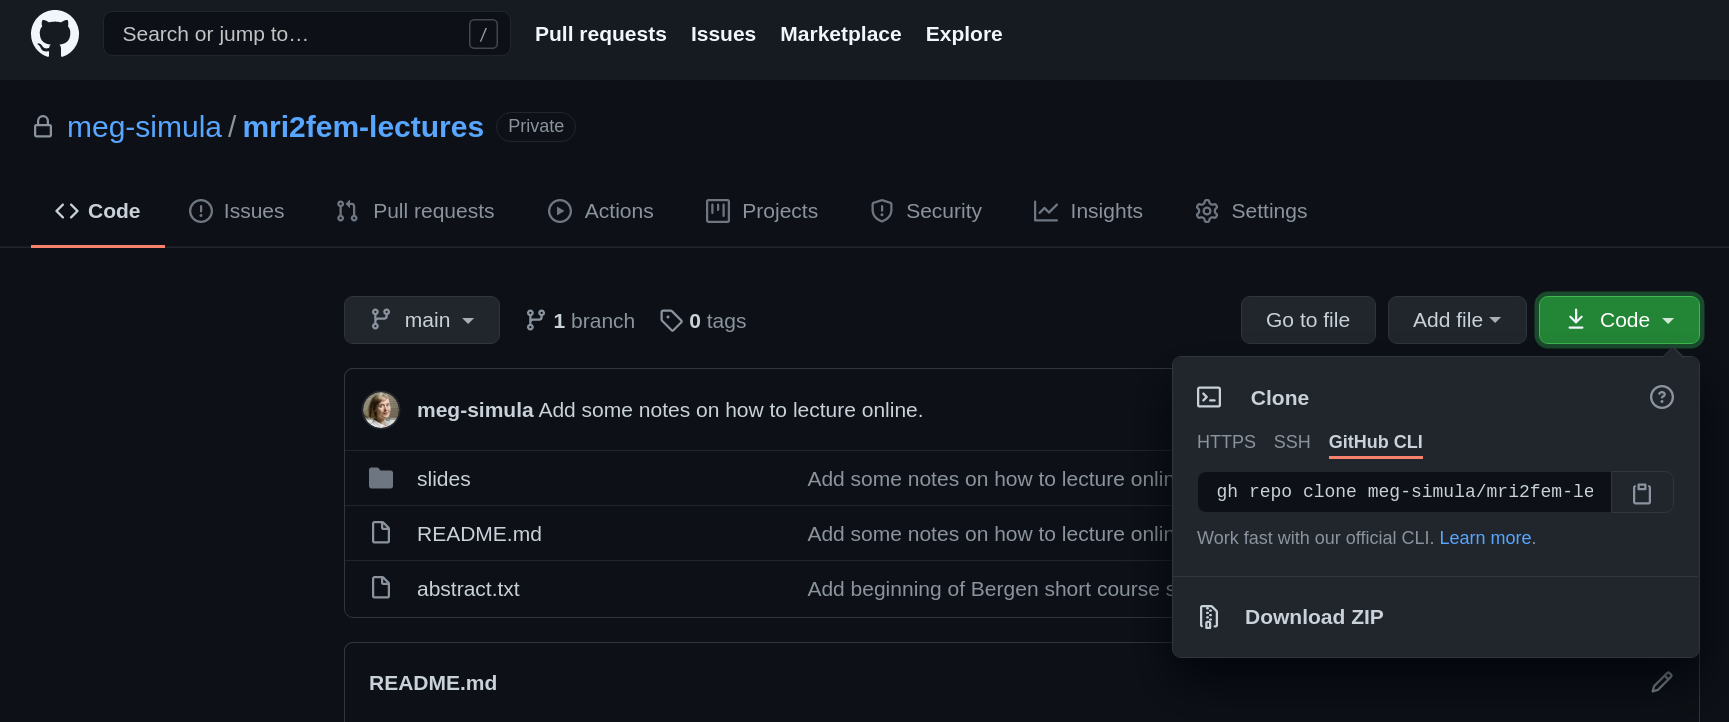
\includegraphics[width=\textwidth]{graphics/mri2fem-lectures-github.png} \\
  \refer{\href{https://github.com/meg-simula/mri2fem-lectures}{https://github.com/meg-simula/mri2fem-lectures}}
}
  
\blackframe{
  \frametitle{Mathematical modeling of the human brain" available on GitHub}
  \framesubtitle{by KA Mardal, ME Rognes, TB Thompson and LM Valnes; Simula SpringerBrief on Computing (2021)}

  \begin{columns}[T]
    \begin{column}{0.3\textwidth}
    \end{column}
    \begin{column}{0.7\textwidth}
    \end{column}
  \end{columns}

  \centering
  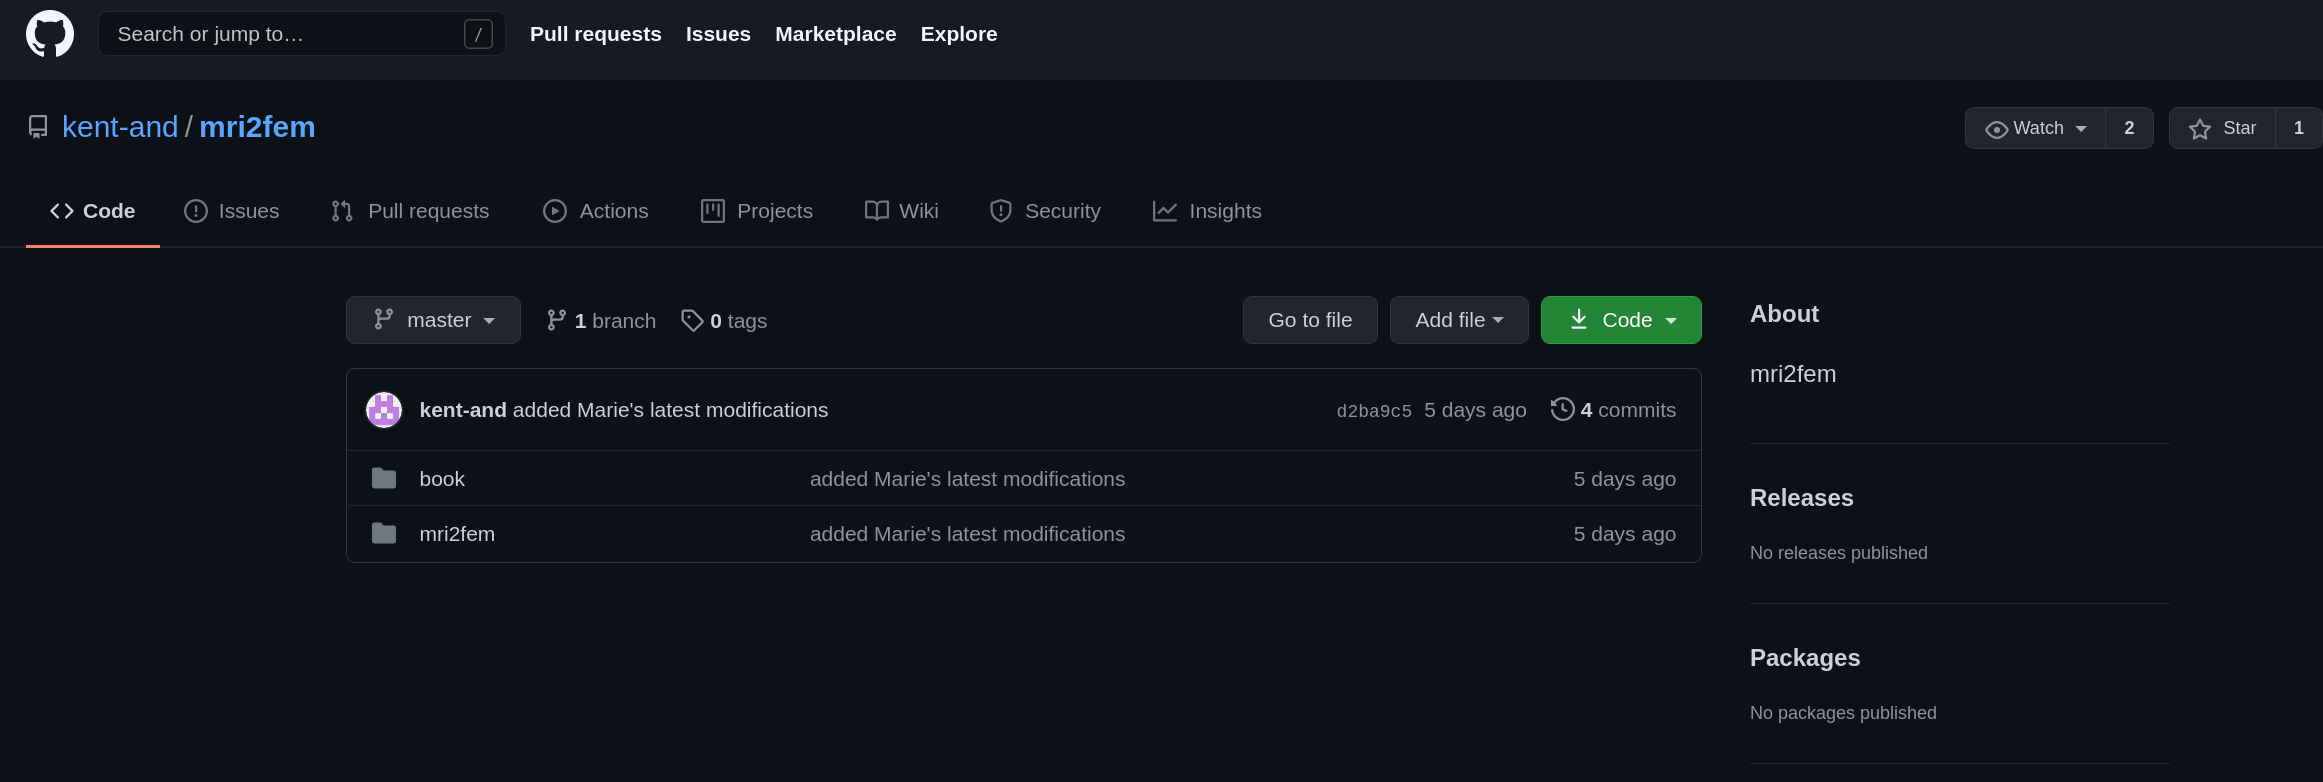
\includegraphics[width=\textwidth]{graphics/mri2fem-book-github.png} \\
  \refer{Mardal et al (2021): \href{https://github.com/kent-and/mri2fem}{https://github.com/kent-and/mri2fem}}
}
  

\begin{frame}
  \frametitle{Resources (data, software) are openly available with our Zenodo community}
  \vspace{-0.5em}
  \centering
  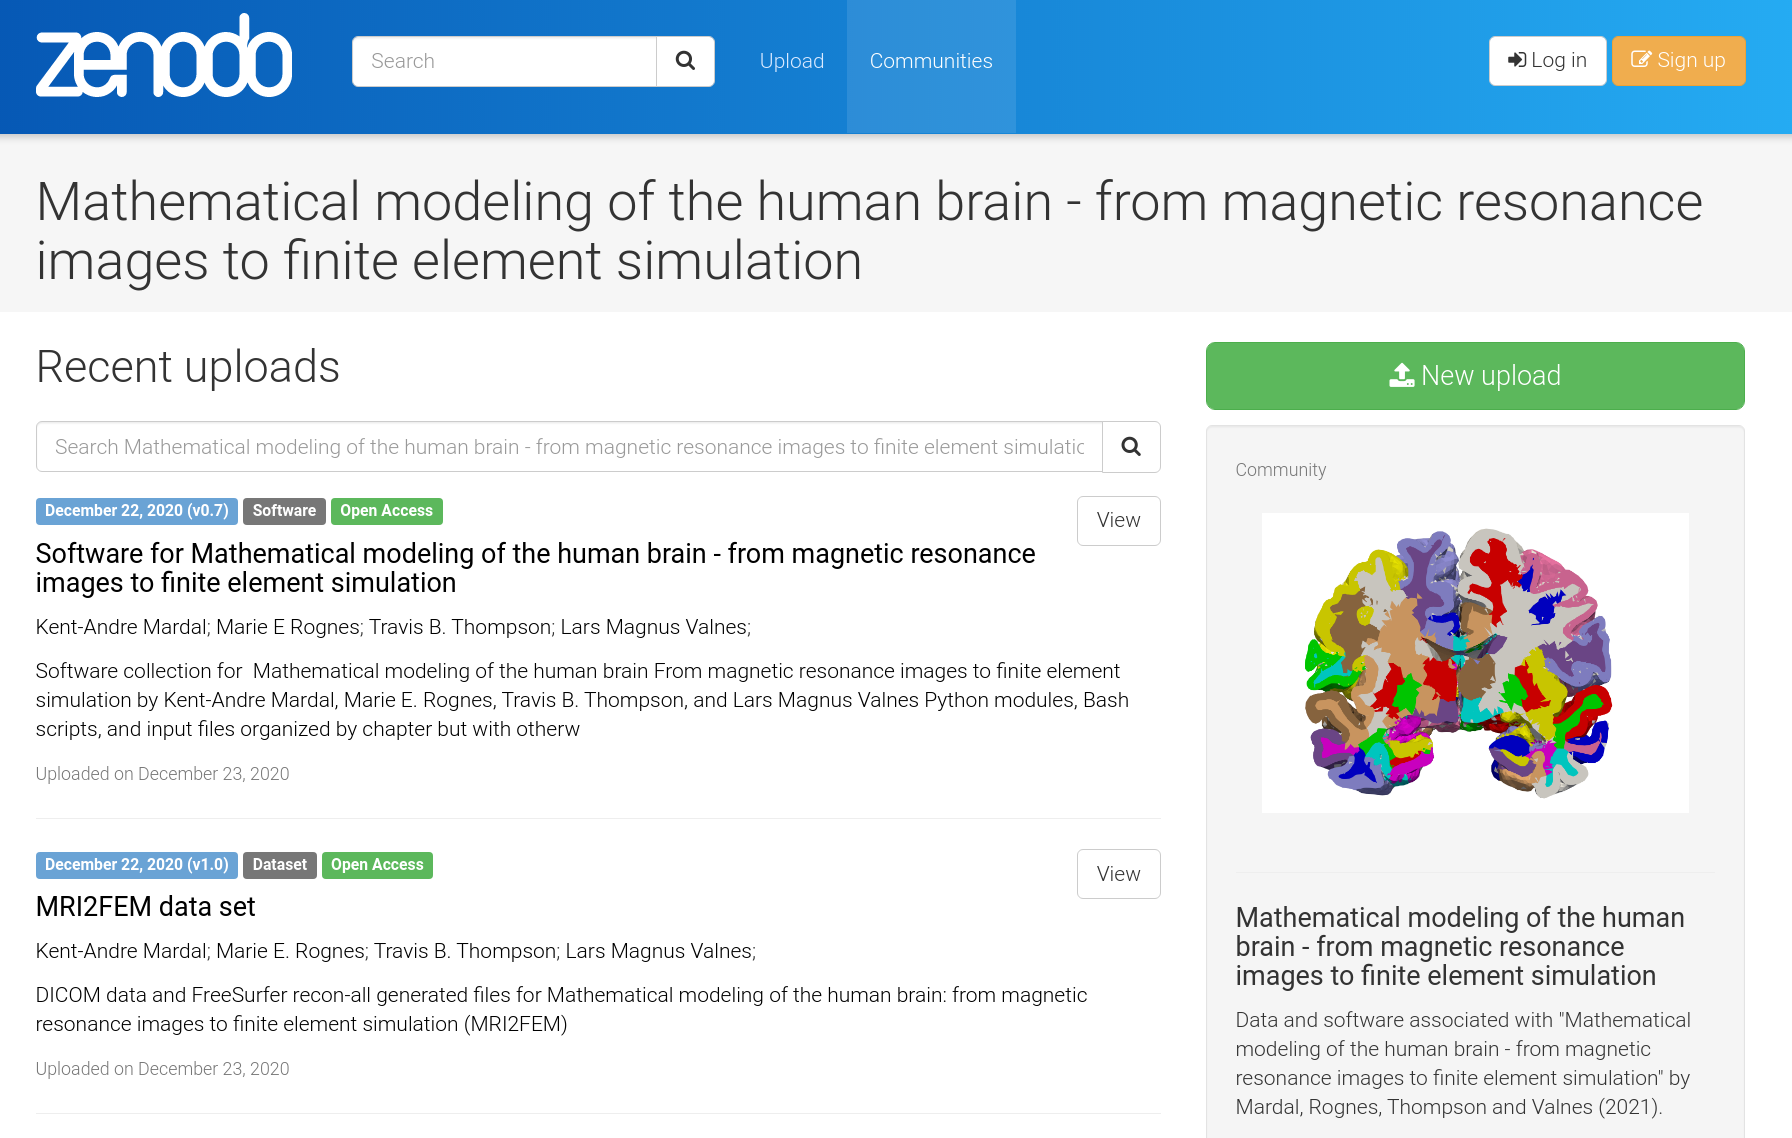
\includegraphics[width=0.85\textwidth]{graphics/mri2fem-zenodo.png} \\
  \vspace{-1em}
  \refer{\href{https://zenodo.org/communities/mri2fem/}{https://zenodo.org/communities/mri2fem/}}
\end{frame}

\begin{frame}
  \frametitle{T1-weighted MRI reveals brain structure}
  \begin{center}
  \includegraphics[height=0.52\textheight]{/home/meg/papers/published/mri2fem/book/graphics/chp2/T1-image.png}
  \includegraphics[height=0.52\textheight]{/home/meg/papers/published/mri2fem/book/graphics/chp2/exp-brain.png}
  \includegraphics[height=0.52\textheight]{/home/meg/papers/published/mri2fem/book/graphics/chp2/exp-matters.png}
  \end{center}

  Axial, sagittal and coronal cross-sections. T1w MRI: fat gives high
  signal intensity (light/white); fluids give low signal intensity
  (dark/black).
\end{frame}

\begin{frame}
  \frametitle{T2-weighted MRI reveals brain structure and fluids}
\begin{figure}
  \centering
  \includegraphics[height=0.7\textheight]{/home/meg/papers/published/mri2fem/book/graphics/chp2/T1-image.png}
  \hspace{2em}
  \includegraphics[height=0.7\textheight]{/home/meg/papers/published/mri2fem/book/graphics/chp2/T2-image.png}
\end{figure}
T1w (left) versus T2w (right). In T2w MRI: fluids gives high signal intensity (light/white)
\end{frame}

\begin{frame}
  \frametitle{Diffusion-tensor MRI reveals water movement and directionality}
  \begin{center}
  \includegraphics[width=0.4\textwidth]{/home/meg/papers/published/mri2fem/book/graphics/chp2/DTI-slice-image-crop.png}
  \hspace{2em}
  \includegraphics[width=0.4\textwidth]{/home/meg/papers/published/mri2fem/book/graphics/chp5/fiber-fa-2.png}
  \end{center}
  In DTI: high signal intensity indicates high degree of anisotropy 
\end{frame}

\begin{frame}
  \frametitle{Viewing and working with MRI data sets in DICOM format}

  Medical images are often stored in the DICOM file format: a
  collection of image files arranged in sequences. A DICOM viewer is
  useful for working with DICOM files.

  \bigskip
  
  Many possibilities including the basic \href{https://wiki.xnat.org/xnat-tools/dicombrowser}{DicomBrowser}

  \bigskip
  
  \terminal{\$ sudo apt-get install dicombrowser \hfill(my Ubuntu 18.04)\\
  \$ DicomBrowser \&}
\end{frame}

\videosection{Video example: downloading and viewing the mri2fem DICOM data set}{https://youtu.be/gvc1owRl-zA}

\begin{frame}
\frametitle{Recommended software components}

\begin{itemize}
\item
  Python3 for everything
\item
  FreeSurfer for segmentation: \href{https://surfer.nmr.mgh.harvard.edu/}{https://surfer.nmr.mgh.harvard.edu/}
\item
  NiBabel for image manipulations: \href{https://nipy.org/nibabel/}{https://nipy.org/nibabel/}
\item
  SVM-Tk for meshing: \href{https://github.com/SVMTK/SVMTK}{https://github.com/SVMTK/SVMTK}
\item
  meshio for mesh conversions: \href{https://github.com/nschloe/meshio}{https://github.com/nschloe/meshio}
\item
  FEniCS for finite elements : \href{https://fenicsproject.org/}{https://fenicsproject.org/}
\item
  ParaView for visualization: \href{https://www.paraview.org/}{https://www.paraview.org/}
\end{itemize}

  \begin{center}
  \includegraphics[height=2.3cm]{/home/meg/papers/published/mri2fem/book/graphics/chp1/T1-image-rot-white.png}
  \includegraphics[height=2.3cm]{/home/meg/papers/published/mri2fem/book/graphics/chp1/ernie-volume-64.png}
  \includegraphics[height=2.3cm]{/home/meg/papers/published/mri2fem/book/graphics/chp1/soltn-t30-crop.png}
  \end{center}


\end{frame}

\begin{frame}
\frametitle{We follow these three steps to generate a mesh from T1 images}

To generate a mesh from an MRI data set including T1-weighted images,
we follow three main steps:
\bigskip
\begin{enumerate}
\item
  extract a T1-weighted image series from the MRI dataset using DicomBrowser;
\item
  create (boundary) surfaces from the T1-weighted images using FreeSurfer;
\item 
  generate a volume mesh of the interior of these using SVM-Tk.
\end{enumerate}
\end{frame}

\begin{frame}
\frametitle{Step 2: Using FreeSurfer to segment images and create surfaces}

FreeSurfer offers the command \emp{recon-all} to segment the brain
images and reconstruct surfaces (parcellations, pial surface, white
matter surface etc.)

\terminal{\$ cd mri2fem-dataset \\
\$ cd dicom/ernie/T13D \\
\$ recon-all -subjid ernie -i IM\_0162 -all}

This command is compute-intensive, with run times likely of 12--24
hours.

Key outputs (\emp{mri2fem-dataset/freesurfer/ernie}) are 
\begin{itemize}
\item \emp{/stats}: contains files providing statistics derived during segmentation.
\item \emp{/mri}: contains volume files generated during segmentation
\item \emp{/surf}: contains surface files generated during segmentation
\end{itemize}
\end{frame}

\videosection{Video example: viewing the FreeSurfer output}{https://youtu.be/Svz3kYfsCQo}
{\terminal{\$ cd mri2fem-dataset/freesurfer/ernie/surf \\
\$ freeview \# Open lh.pial \\
\$ \\
\$ mris\_convert ./lh.pial pial.stl \\
\$ paraview \# Open lh.pial.stl}
}


\begin{frame}
\frametitle{The surfaces may need enhancement to be suitable for finite element meshes}

\begin{columns}[T]
\begin{column}{0.6\textwidth}
In practice, brain surfaces generated from T1 images 
\begin{itemize}
\item may have unphysiologically sharp corners,   
\item may include triangles with very large aspect ratios, 
\item have topological defects such as holes, and
\item may self-intersect or overlap with other surfaces.   
\end{itemize}

\medskip

\alert{Result:} Low quality meshes (if any). \\

\medskip

\alert{Fix:} Enhance surface quality prior to meshing
\end{column}
\begin{column}{0.4\textwidth}
  \centering
  \includegraphics[width=\textwidth]{/home/meg/papers/published/mri2fem/book/graphics/chp3/juncturers-gap.png}
\end{column}

\end{columns}
\end{frame}


\begin{frame}
  \frametitle{SVM-Tk (wrapping CGAL) includes utilities for remeshing surfaces}
  \centering
  \includegraphics[width=0.49\textwidth]{/home/meg/papers/published/mri2fem/book/graphics/chp3/raw-stlmesh.png}
  \includegraphics[width=0.49\textwidth]{/home/meg/papers/published/mri2fem/book/graphics/chp3/remesh-stlmesh.png}
  \refer{Mardal et al (2021, Chapter 3.2.1); \href{https://github.com/kent-and/mri2fem/blob/master/mri2fem/mri2fem/chp3/remesh_surface.py}{mri2fem/chp3/remesh\_surface.py}}
\end{frame}


\begin{frame}
  \frametitle{SVM-Tk includes utilities for smoothing surfaces}
  \begin{figure}
  \centering
  \includegraphics[width=0.32\textwidth]{/home/meg/papers/published/mri2fem/book/graphics/chp3/unsmoothed.png}
  \includegraphics[width=0.32\textwidth]{/home/meg/papers/published/mri2fem/book/graphics/chp3/taubin-smoothed-10.png}
  \includegraphics[width=0.32\textwidth]{/home/meg/papers/published/mri2fem/book/graphics/chp3/oversmoothing.png}

  Original pial surface \hspace{3em} after Taubin smoothing \hspace{3em}
after over-smoothing.
  \end{figure}
  \bigskip
  
  \refer{Mardal et al (2021, Chapter 3.2.2); \href{https://github.com/kent-and/mri2fem/blob/master/mri2fem/mri2fem/chp3/smooth_surface.py}{mri2fem/chp3/smooth\_surface.py}}
\end{frame}

\begin{frame}[fragile]
\frametitle{SVM-Tk is designed to create brain volume meshes from surfaces}

\begin{columns}
\begin{column}{0.34\textwidth}
\begin{figure}
  \centering
  \includegraphics[width=\textwidth]{/home/meg/papers/published/mri2fem/book/graphics/chp3/ernie-volume-16-r.png} \\
  \includegraphics[width=\textwidth]{/home/meg/papers/published/mri2fem/book/graphics/chp3/ernie-volume-64-r.png}
\end{figure}
\end{column}
\begin{column}{0.65\textwidth}
  \begin{python}
import SVMTK as svmtk

def create_volume_mesh(stlfile, output, n=16):
    # Load input file
    surface = svmtk.Surface(stlfile)
    
    # Generate the volume mesh
    domain = svmtk.Domain(surface)
    domain.create_mesh(n)

    # Write the mesh to the output file
    domain.save(output)

# Create mesh    
create_volume_mesh("lh.pial.stl", "lh.mesh")
  \end{python}
  \refer{Mardal et al (2021, Chapter 3.1.3); \href{https://github.com/kent-and/mri2fem/blob/master/mri2fem/mri2fem/chp3/surface_to_mesh.py}{mri2fem/chp3/surface\_to\_mesh.py}}
\end{column}
\end{columns}

\end{frame}

\videosection{Video example: creating a mesh of the left hemisphere}{https://youtu.be/tHGmzPqiYhQ}

\input{/home/meg/presentations/slidesx/mri2fem_parcellations.tex}

\videosection{Video example: simulating diffusion using FEniCS}{https://youtu.be/zs_vcLFfPFk}

\begin{frame}
\frametitle{Igor, bring me the brain! Want to give it a try? Natural first steps:}
\begin{enumerate}
\item
  Download the slides from this lecture:  \href{https://github.com/meg-simula/mri2fem-lectures}{https://github.com/meg-simula/mri2fem-lectures}.
\item
  Download the mri2fem data set and software from Zenodo and inspect
  the contents using the tools discussed.
\item
  Download the book: Mardal et al (2021): \href{https://github.com/kent-and/mri2fem}{https://github.com/kent-and/mri2fem}.
\item
  Install software dependencies following the instructions in Chapter
  2 of Mardal et al (2021).
\item
  Try running some of the sample code in Chapter 3 of Mardal et al
  (2021).
\item
  Simulate something other than diffusion? Give it a try!
\end{enumerate}
\end{frame}


\mysection{Concluding remarks}

\input{/home/meg/presentations/slidesx/research_overview.tex}

{\usebackgroundtemplate{\includegraphics[width=\paperwidth]{graphics/Collaborators2022.pdf}}
  \begin{frame}
  \end{frame}
}

\end{document}


